%%%%%%%%%%%%%%%%%%%%%%%%%%%%%%%%%%%%%%%%%
% Beamer Presentation
% LaTeX Template
% Version 1.0 (10/11/12)
%
% This template has been downloaded from:
% http://www.LaTeXTemplates.com
%
% License:
% CC BY-NC-SA 3.0 (http://creativecommons.org/licenses/by-nc-sa/3.0/)
%
%%%%%%%%%%%%%%%%%%%%%%%%%%%%%%%%%%%%%%%%%

%----------------------------------------------------------------------------------------
%   PACKAGES AND THEMES
%----------------------------------------------------------------------------------------

%\documentclass{beamer}
\documentclass[aspectratio=169]{beamer}
\mode<presentation> {

  % The Beamer class comes with a number of default slide themes
  % which change the colors and layouts of slides. Below this is a list
  % of all the themes, uncomment each in turn to see what they look like.

  %\usetheme{default}
  %\usetheme{AnnArbor}
  %\usetheme{Antibes}
  %\usetheme{Bergen}
  %\usetheme{Berkeley}
  %\usetheme{Berlin}
  %\usetheme{Boadilla}
  %\usetheme{CambridgeUS}
  %\usetheme{Copenhagen}
  %\usetheme{Darmstadt}
  %\usetheme{Dresden}
  %\usetheme{Frankfurt}
  %\usetheme{Goettingen}
  %\usetheme{Hannover}
  %\usetheme{Ilmenau}
  %\usetheme{JuanLesPins}
  %\usetheme{Luebeck}
  \usetheme{Madrid}
  %\usetheme{Malmoe}
  %\usetheme{Marburg}
  %\usetheme{Montpellier}
  %\usetheme{PaloAlto}
  %\usetheme{Pittsburgh}
  %\usetheme{Rochester}
  %\usetheme{Singapore}
  %\usetheme{Szeged}
  %\usetheme{Warsaw}

  % As well as themes, the Beamer class has a number of color themes
  % for any slide theme. Uncomment each of these in turn to see how it
  % changes the colors of your current slide theme.

  %\usecolortheme{albatross}
  %\usecolortheme{beaver}
  %\usecolortheme{beetle}
  %\usecolortheme{crane}
  %\usecolortheme{dolphin}
  %\usecolortheme{dove}
  %\usecolortheme{fly}
  %\usecolortheme{lily}
  %\usecolortheme{orchid}
  %\usecolortheme{rose}
  %\usecolortheme{seagull}
  %\usecolortheme{seahorse}
  \usecolortheme{whale}
  %\usecolortheme{wolverine}

  %\setbeamertemplate{footline} % To remove the footer line in all slides uncomment this line
  %\setbeamertemplate{footline}[page number] % To replace the footer line in all slides with a simple slide count uncomment this line

  %\setbeamertemplate{navigation symbols}{} % To remove the navigation symbols from the bottom of all slides uncomment this line
}
\usefonttheme[onlymath]{serif}
%\usepackage{epsfig}
\usepackage{graphicx} % Allows including images
\usepackage{booktabs} % Allows the use of \toprule, \midrule and \bottomrule in tables
\usepackage{multimedia} % 
\usepackage{multirow}
%\usepackage{animate}
%\usepackage{tikz}
%\usepackage{lipsum}

\usepackage{tikz} 
\usetikzlibrary{tikzmark,overlay-beamer-styles,positioning,calc}
%\usetikzlibrary{tikzmark,
%\usetikzlibrary{tikzmark}
%\usetikzlibrary{arrows,shapes}
%\newcommand{\tikzmark}[1]{\tikz[remember picture] \node[coordinate] (#1) {#1};}
\newcommand{\be}{\begin{equation*}}
\newcommand{\ee}{\end{equation*}}
\newcommand{\ol}{\overline}
\newcommand{\p}{\partial}
\newcommand{\pdv}[2]{\frac{\partial \, #1}{\partial #2}}
\newcommand{\etal}{ {\it et al.} }
%----------------------------------------------------------------------------------------
%   TITLE PAGE
%----------------------------------------------------------------------------------------

\title[CHARTS]{Candidate CHARTS Model Update} % The short title appears at the bottom of every slide, the full title is only on the title page

\author[]{Brad Johnson\\Liz Holzenthal\\Rusty Permenter \\Kevin Hodgens } % Your name
\institute[ERDC] % Your institution as it will appear on the bottom of every slide, may be shorthand to save space
{USACE Engineering Research and Devlelopment Center \\ % Your institution for the title page
\medskip
\textit{} % Your email address
}
%\date{\today} % Date, can be changed to a custom date
\date{\vspace*{-0cm}\\ Feb, 2025} % Date, can be changed to a custom date

\begin{document}

\begin{frame}
  %\titlepage % Print the title page as the first slide
  \begin{columns}[c] % The "c" option specifies centered vertical alignment while the "t" option is used for top vertical alignment
    
    \column{.3\textwidth} % Left column and width
    \titlepage % Print the title page as the first slide
%%     \vspace*{-1cm}
%%     \begin{center}
%% District PDT:\\
%% Kelly Legault (SAJ)\\
%% Gabriel Todaro (SAJ)
%%     \end{center}
    \column{.7\textwidth} % Right column and width
    \begin{figure}
            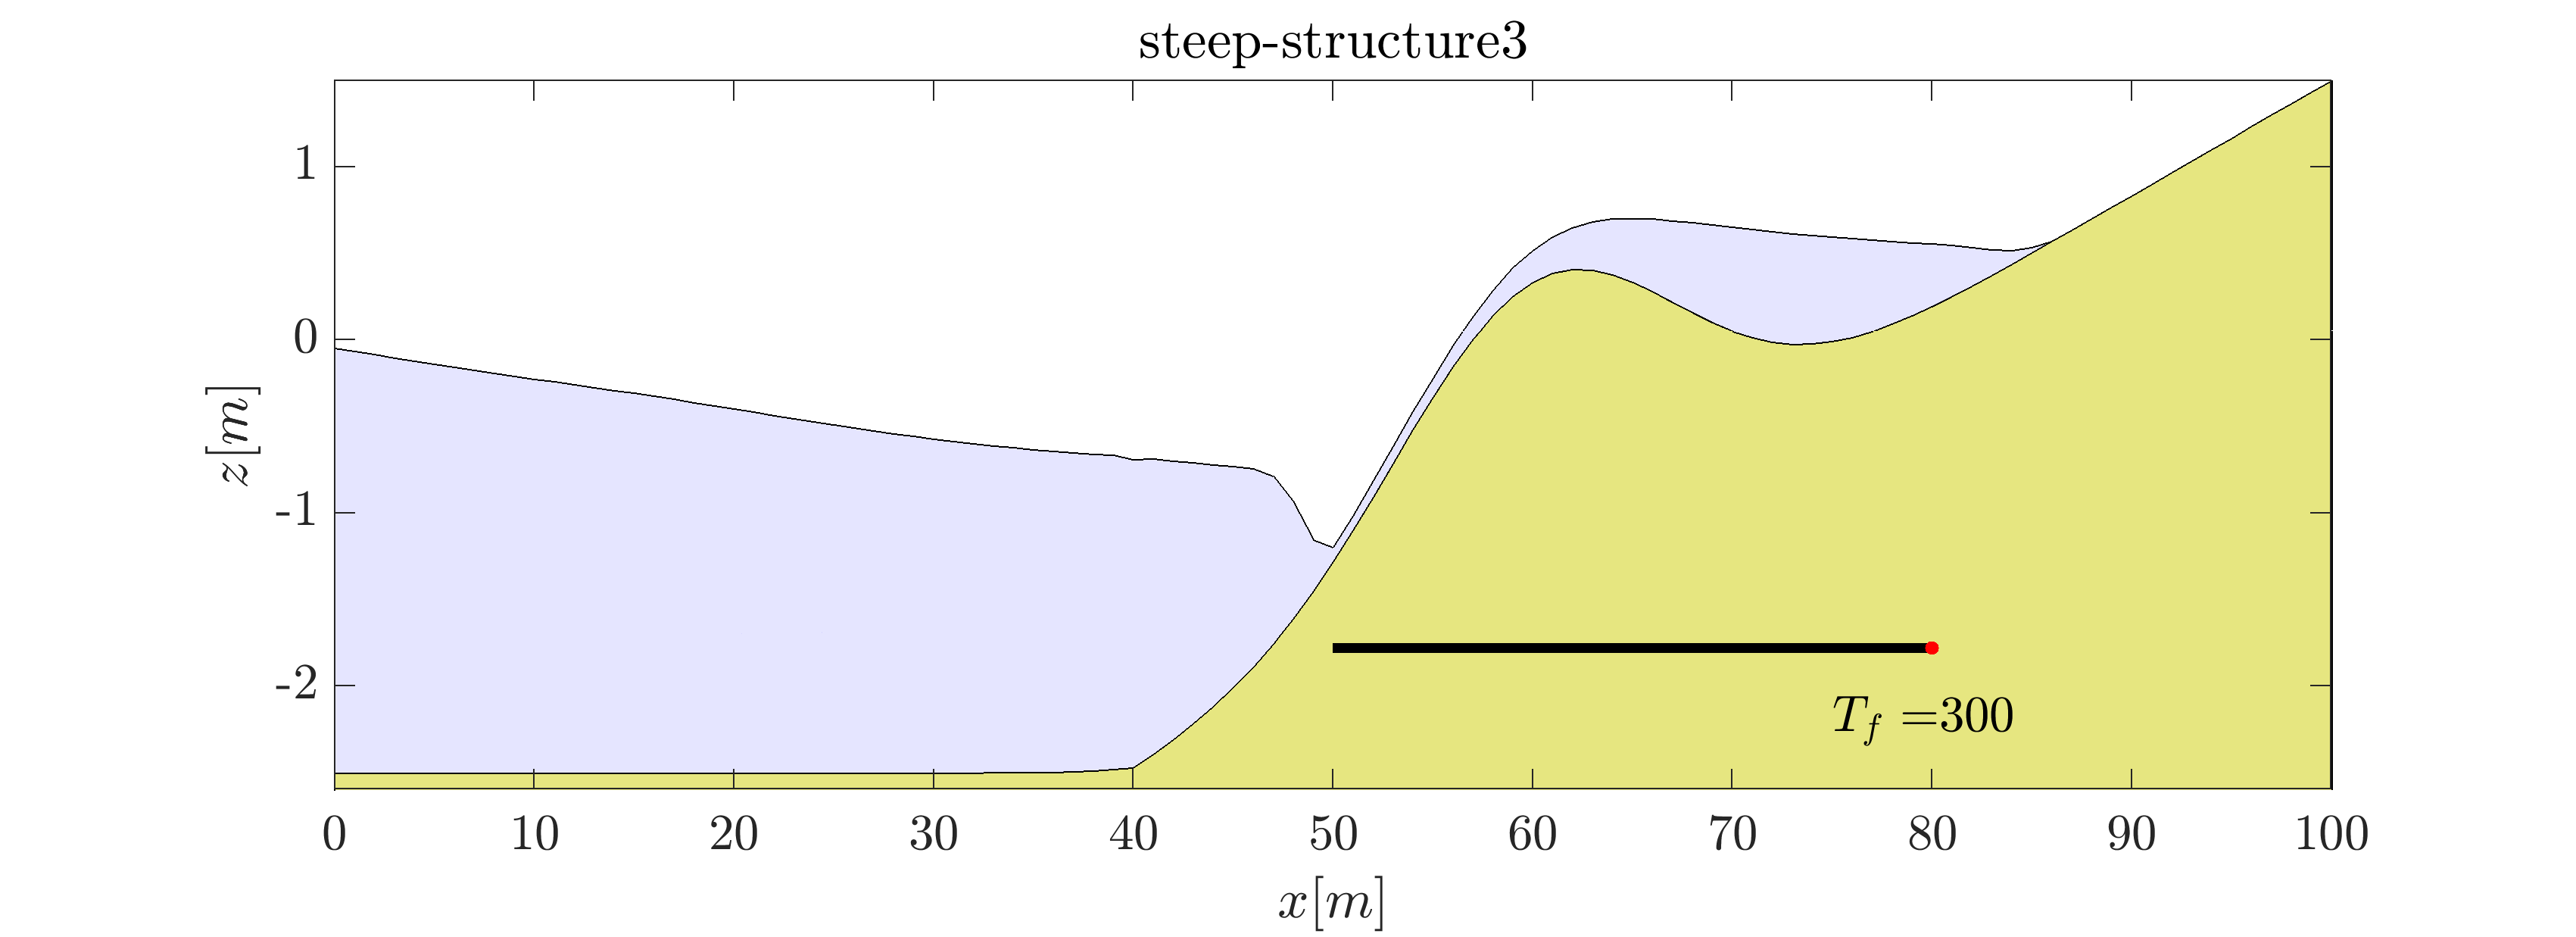
\includegraphics[width=1\linewidth]{./present.png}
      %\includegraphics[trim={0 1cm 0 0},clip,width=0.9\linewidth]{./breaking-wave-on-the-beach.jpg}
    \end{figure}
    
  \end{columns}
\end{frame}

%%%%%%%%%%%%%%%%%%%%%%%%%%%%%%%%%%%%%%%%%%%%%%%%%%%%%%%%%%%%%%%%%%%%%%%%%%%%%%%%%%%%%%%%%%%%%%%%%%%%
\begin{frame}
  \frametitle{Challenges}
  In cases of large slope and super-critical flow (esp with large concavity), challenge with instability  
  \centering
  \movie[externalviewer]{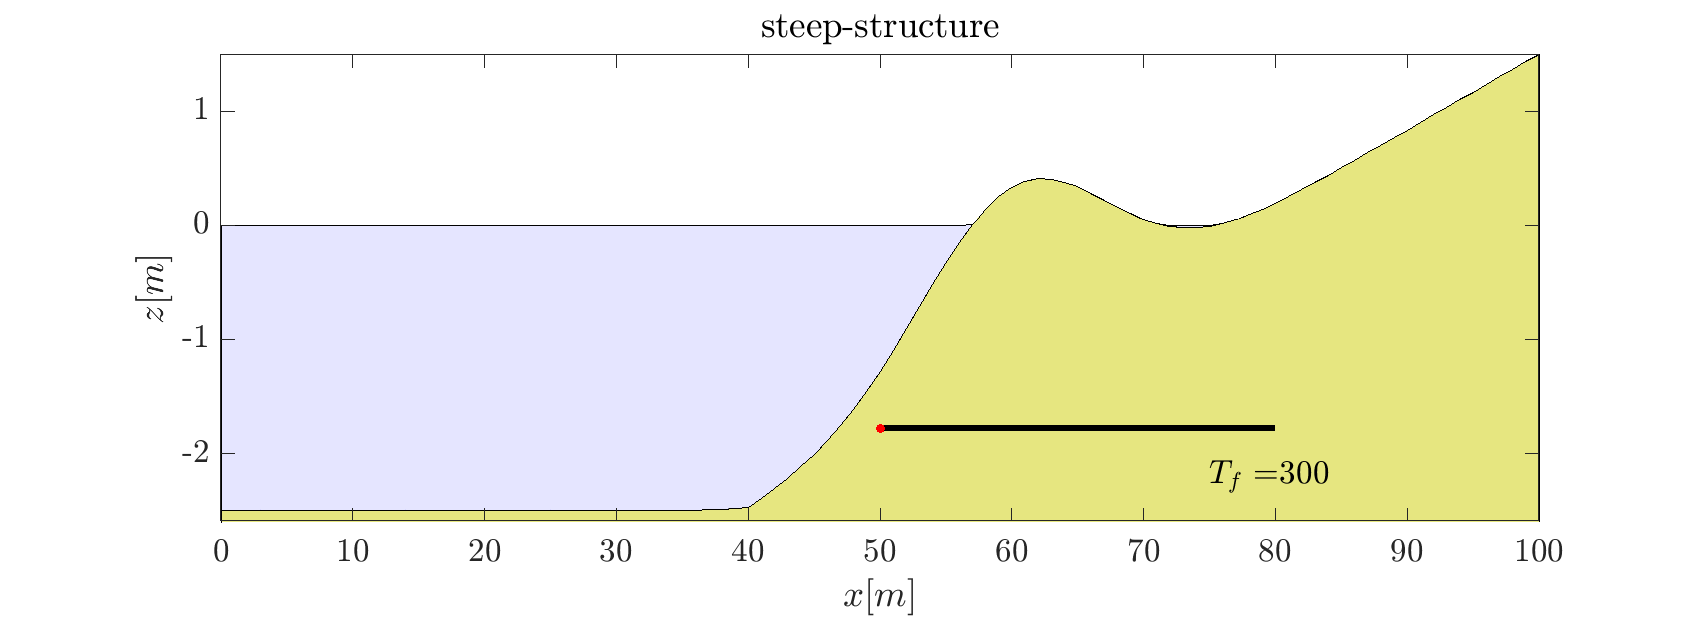
\includegraphics[width=\textwidth, keepaspectratio]
    {./steep_structure.png}}{./steep_structure.avi}
\end{frame}
%%%%%%%%%%%%%%%%%%%%%%%%%%%%%%%%%%%%%%%%%%%%%%%%%%%%%%%%%%%%%%%%%%%%%%%%%%%%%%%%%%%%%%%%%%%%%%%%%%%%
\begin{frame}[fragile]
  \frametitle{New Hydraulic Time-step Integration}
  Within \texttt{shallow\_water\_moving\_shore.m}, integrate in time from time-step $k$ to $k+1$:
   \begin{itemize}
   \item Compute wave transformation and stresses
   \item Predict $q^{k+1}$ on the basis of $q^{k},h^k$ using momentum conservation
   \item \textcolor{blue}{$\hat{q}_i^{k+1} = (1-\nu) q_i^{k+1} + \frac{\nu}{2}(q_{i+1}^{k+1} + q_{i-1}^{k+1})
     \;\;\;\;\;\; 0\leq \nu <0.5 \;\;\;  \mbox{for} \;\;\; max(Fr)>1$}
   \item \textcolor{blue}{$\hat{h}_i^{k} = (1-\nu) h_i^{k} + \frac{\nu}{2}(h_{i+1}^{k} + h_{i-1}^{k}) 
     \;\;\;\;\;\;\;\;\;\;\;\;\; 0\leq \nu <0.5 \;\;\;  \mbox{for} \;\;\; max(Fr)>1$}
   \item \textcolor{blue}{Restore wet/dry conditions that preceded smoothing}
   \item Predict $h^{k+1}$ on the basis of $\hat{q}^{k+1},\hat{h}^k$ using mass conservation
   \end{itemize}
\end{frame}
%%%%%%%%%%%%%%%%%%%%%%%%%%%%%%%%%%%%%%%%%%%%%%%%%%%%%%%%%%%%%%%%%%%%%%%%%%%%%%%%%%%%%%%%%%%%%%%%%%%%
\begin{frame}
  \frametitle{Challenges}
  Making use of $\nu = 0.1$
  \centering
  \movie[externalviewer]{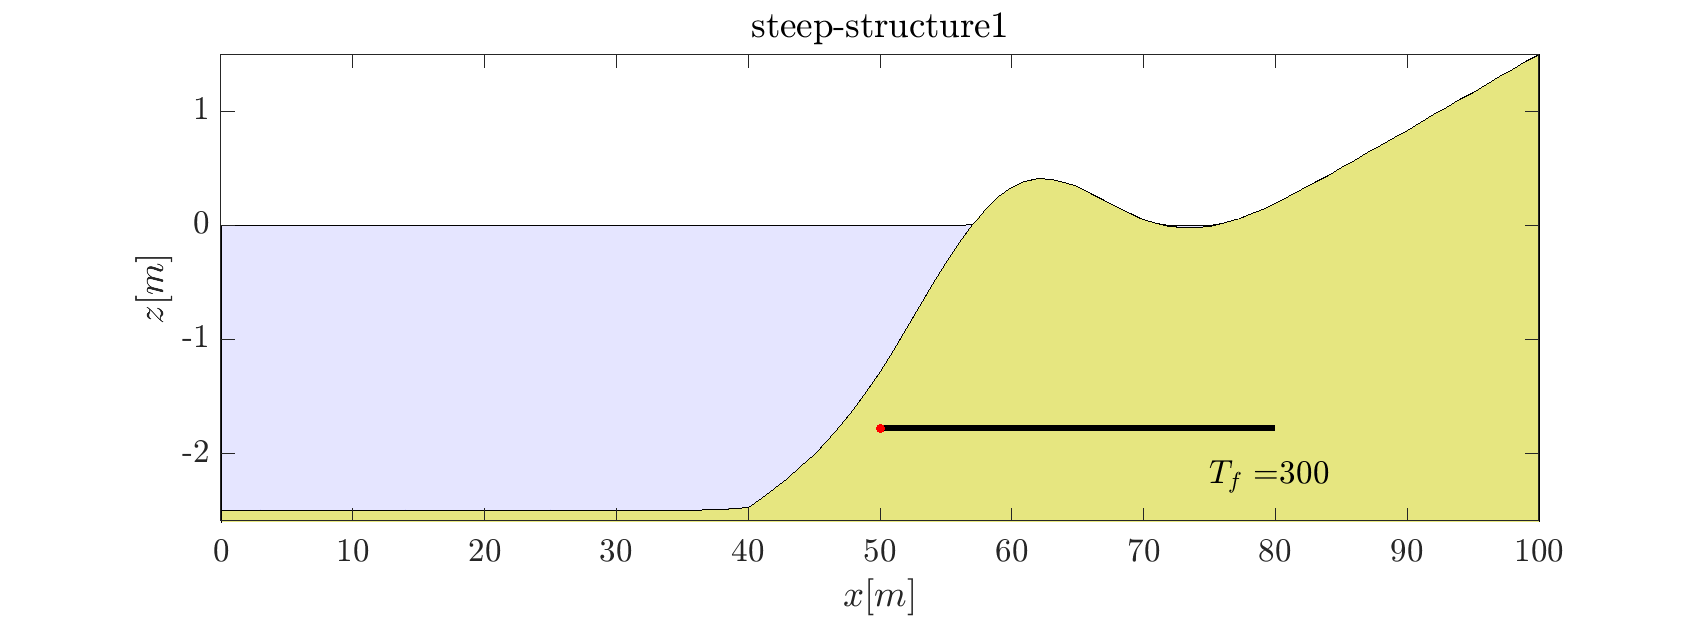
\includegraphics[width=\textwidth, keepaspectratio]
    {./steep_structure1.png}}{./steep_structure1.avi}
\end{frame}
%%%%%%%%%%%%%%%%%%%%%%%%%%%%%%%%%%%%%%%%%%%%%%%%%%%%%%%%%%%%%%%%%%%%%%%%%%%%%%%%%%%%%%%%%%%%%%%%%%%%
\begin{frame}
  \frametitle{Challenges}
  Making use of $\nu = 0.2$
  \centering
  \movie[externalviewer]{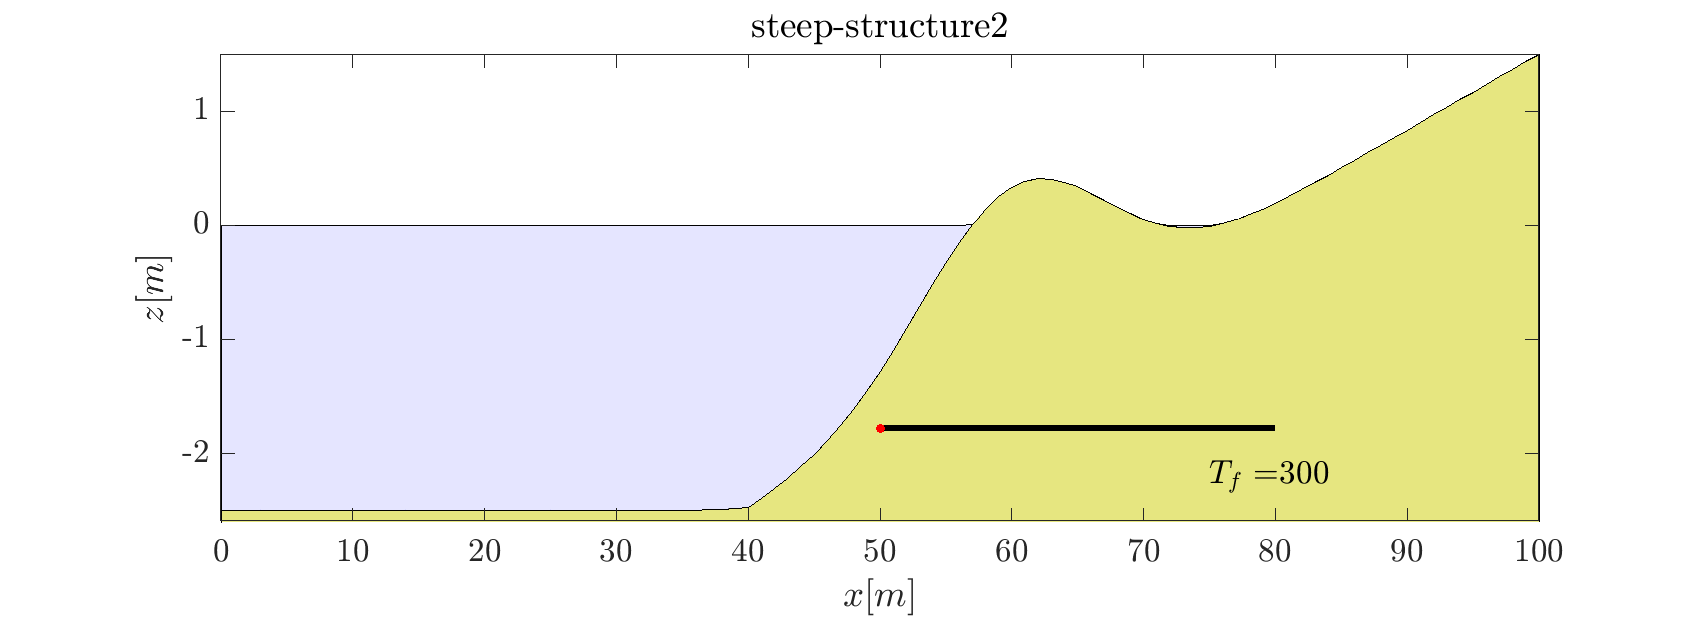
\includegraphics[width=\textwidth, keepaspectratio]
    {./steep_structure2.png}}{./steep_structure2.avi}
\end{frame}
%%%%%%%%%%%%%%%%%%%%%%%%%%%%%%%%%%%%%%%%%%%%%%%%%%%%%%%%%%%%%%%%%%%%%%%%%%%%%%%%%%%%%%%%%%%%%%%%%%%%
\begin{frame}
  \frametitle{Challenges}
  Making use of $\nu = 0.3$
  \centering
  \movie[externalviewer]{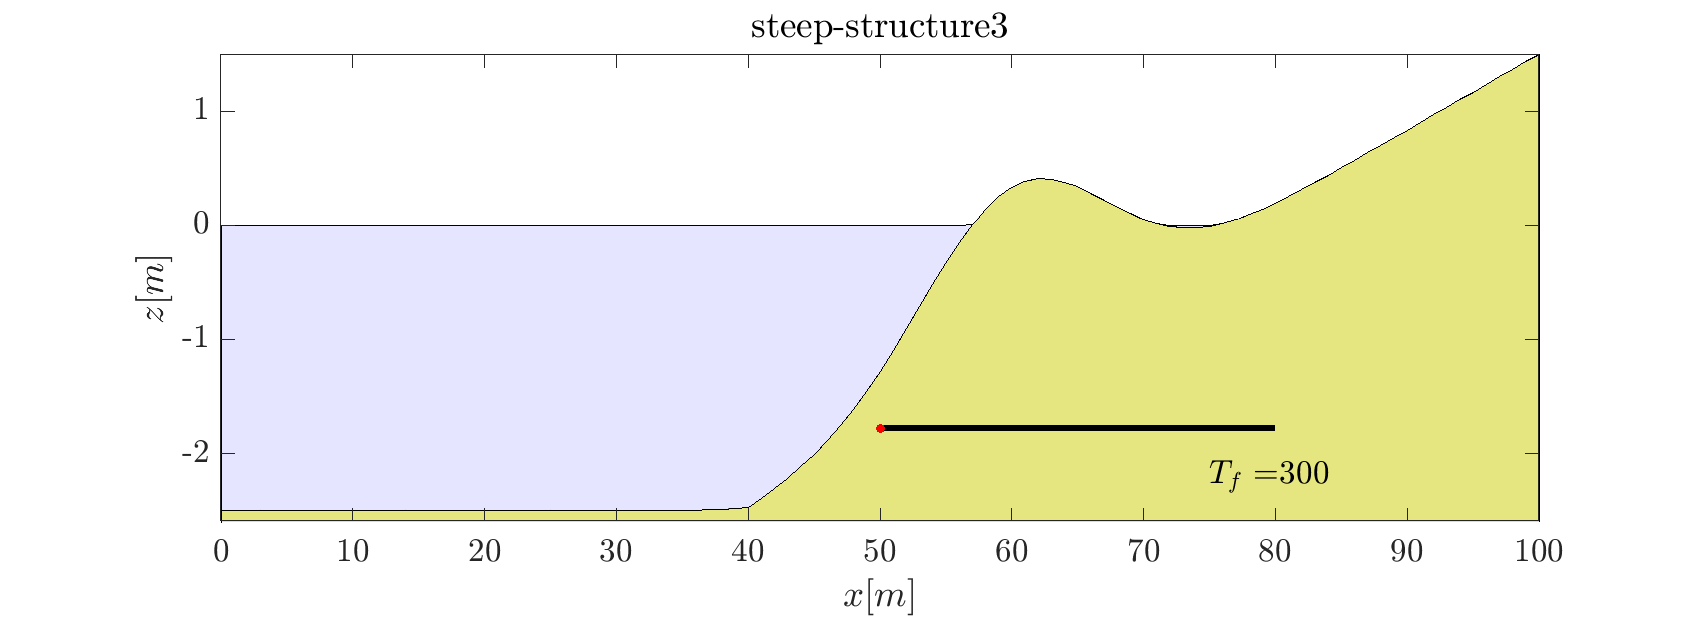
\includegraphics[width=\textwidth, keepaspectratio]
    {./steep_structure3.png}}{./steep_structure3.avi}
\end{frame}
%%%%%%%%%%%%%%%%%%%%%%%%%%%%%%%%%%%%%%%%%%%%%%%%%%%%%%%%%%%%%%%%%%%%%%%%%%%%%%%%%%%%%%%%%%%%%%%%%%%%

\begin{frame}
  \frametitle{CHARTS Morphology Component Options }
  \small
  All model Challenges:
  \begin{itemize}
  \item Usability: e.g. GUI including MC. etc 
  \item Combining erosive/accretionary modes
    \item Logistics: e.g. Programming language, OS independence, etc  
  \end{itemize}

      
\begin{table}[h]
  \begin{center}
    \begin{tabular}{l|l|l|l}
     \textbf{Model} & \textbf{Deficiency} & \textbf{Remedy} & \textbf{Risk}\\
      \hline
      \multirow{3}{*}{CSHORE} & Hard-bottom & Recast sand conservation& Moderate/High\\ % <--
      & Upland dynamics&Dev/Code improvement& Moderate\\ % <--
      & Lacks 2DH &Dev& Moderate\\ % <-- 
      \hline
      \multirow{4}{*}{CHANLSW}& Swash characterization & Develop closure& Low/Moderate\\ % <-- C
      & Computational efficiency& ?GPU?& Moderate/High\\ % <-- Content of first column omitted.
      & Morpho not verified& Comp model/data & Moderate/High\\ % <-- Content of first column omitted.
      & Lacks 2DH &Dev& Moderate\\ % <--
      \hline
      \multirow{2}{*}{2DH: D3D CMS}   & Upland dynamics & None&\\ % <-- Combining 2 rows with arbitrary with (*) and content 12
                              & Computational Efficiency& ML& High\\ % <-- Content of first column omitted.
      \hline
      \multirow{1}{*}{2DH:XBeach} & Computational Efficiency& ML& High\\ % <-- Content of first column omitted.
      \hline
    \end{tabular}
  \end{center}
\end{table}

\end{frame}
%%%%%%%%%%%%%%%%%%%%%%%%%%%%%%%%%%%%%%%%%%%%%%%%%%%%%%%%%%%%%%%%%%%%%%%%%%%%%%%%%%%%%%%%%%%%%%%%%%%%
  
\end{document}
